
\subsection{Motivation and Relevance}

Noise emissions from air traffic in areas close to airports is a constant battle. The new aero-engines in development at Rolls-Royce, General Electric, and Pratt \& Whitney have increasingly larger bypass ratios to increase overall efficiency. This ultimately leads to larger fans and a growth in nacelle diameter. Previously, engine manufacturers have simply increased the inlet and bypass lengths proportionally with the nacelle diameter, but the associated drag and weight penalties of doing this for next generation engines is unfeasible. Therefore, there is physically less nacelle space for acoustic liners, requiring more efficient liner damping to meet emissions regulations. Compounding this is the fact that larger engines produce lower blade passing frequencies (BPF) which require deeper liners to attenuate the noise, and thus thicker nacelles. This is again not possible due to drag and weight penalties. So new, highly-complex liner concepts are required. An example of such a liner is the Special Acoustic Absorber (SAA), developed by \textcite{redmann2013aeroacousticliner} in 2013. The added complexity of these new liners enforces the need for CAA solvers with clever features, such as efficient non-reflecting boundary conditions (NRBCs). These features are parameterised to the effect that specific combinations of parameters impact the accuracy of the resolved wave propagation inside the domain. 



\subsection{General Aim and Scope}
The primary aim of this project is to investigate a specific non-reflecting boundary condition (NRBC) formulation for use in truncating a computational aeroacoustics domain. The aim is constituted of a number of objectives, including:

\begin{enumerate}
\itemsep0em
\item Accurately \textbf{discretise} complex \textbf{PDEs} using CAA-relevant schemes - governing Euler equations require discretising in space and time using aeroacoustic-optimised formulations
\item Write a \textbf{linearised solver} in MATLAB to predict wave propagation problems - commercial solvers do not yet offer enough flexibility for integrating innovative BCs
\item Implement absorbing zone \textbf{NRBCs}
\item \textbf{Benchmark} the solver against \textbf{workshop problems} - NASA-published aeroacoustics workshops for solver validation
\item Determine \textbf{optimal parameters} for the NRBC implementation - considering induced-error from combinations of parameters
\end{enumerate}

The listed objectives ensure a rigorous and thorough approach that delivers tangible results. 

\newpage

\subsection{Design Context}


The 'optimised' boundary condition parameters sought after in this report could be used in a more matured research solver for exploring unique and innovative acoustic liners. The potential cash impact, then, is two-fold. Firstly computational expenses are reduced by using efficient BC parameters - as less grid points are solved. Secondly, costs can be cut by decreasing drag and weight, which is enabled by shorter/thinner nacelles, which is enabled by space-efficient liners, which is enabled by accurate cutting-edge CAA methods. The end result is beneficial in both a holistic and cash sense.


\subsection{Report Structure and Conventions}

The report structure is illustrated in Figure \ref{fig:ReportStructure}, and follows a rough layout of background \& literature review, methodology, results, and conclusion. 

\begin{figure}[h!]
\centering
\makebox[0pt]{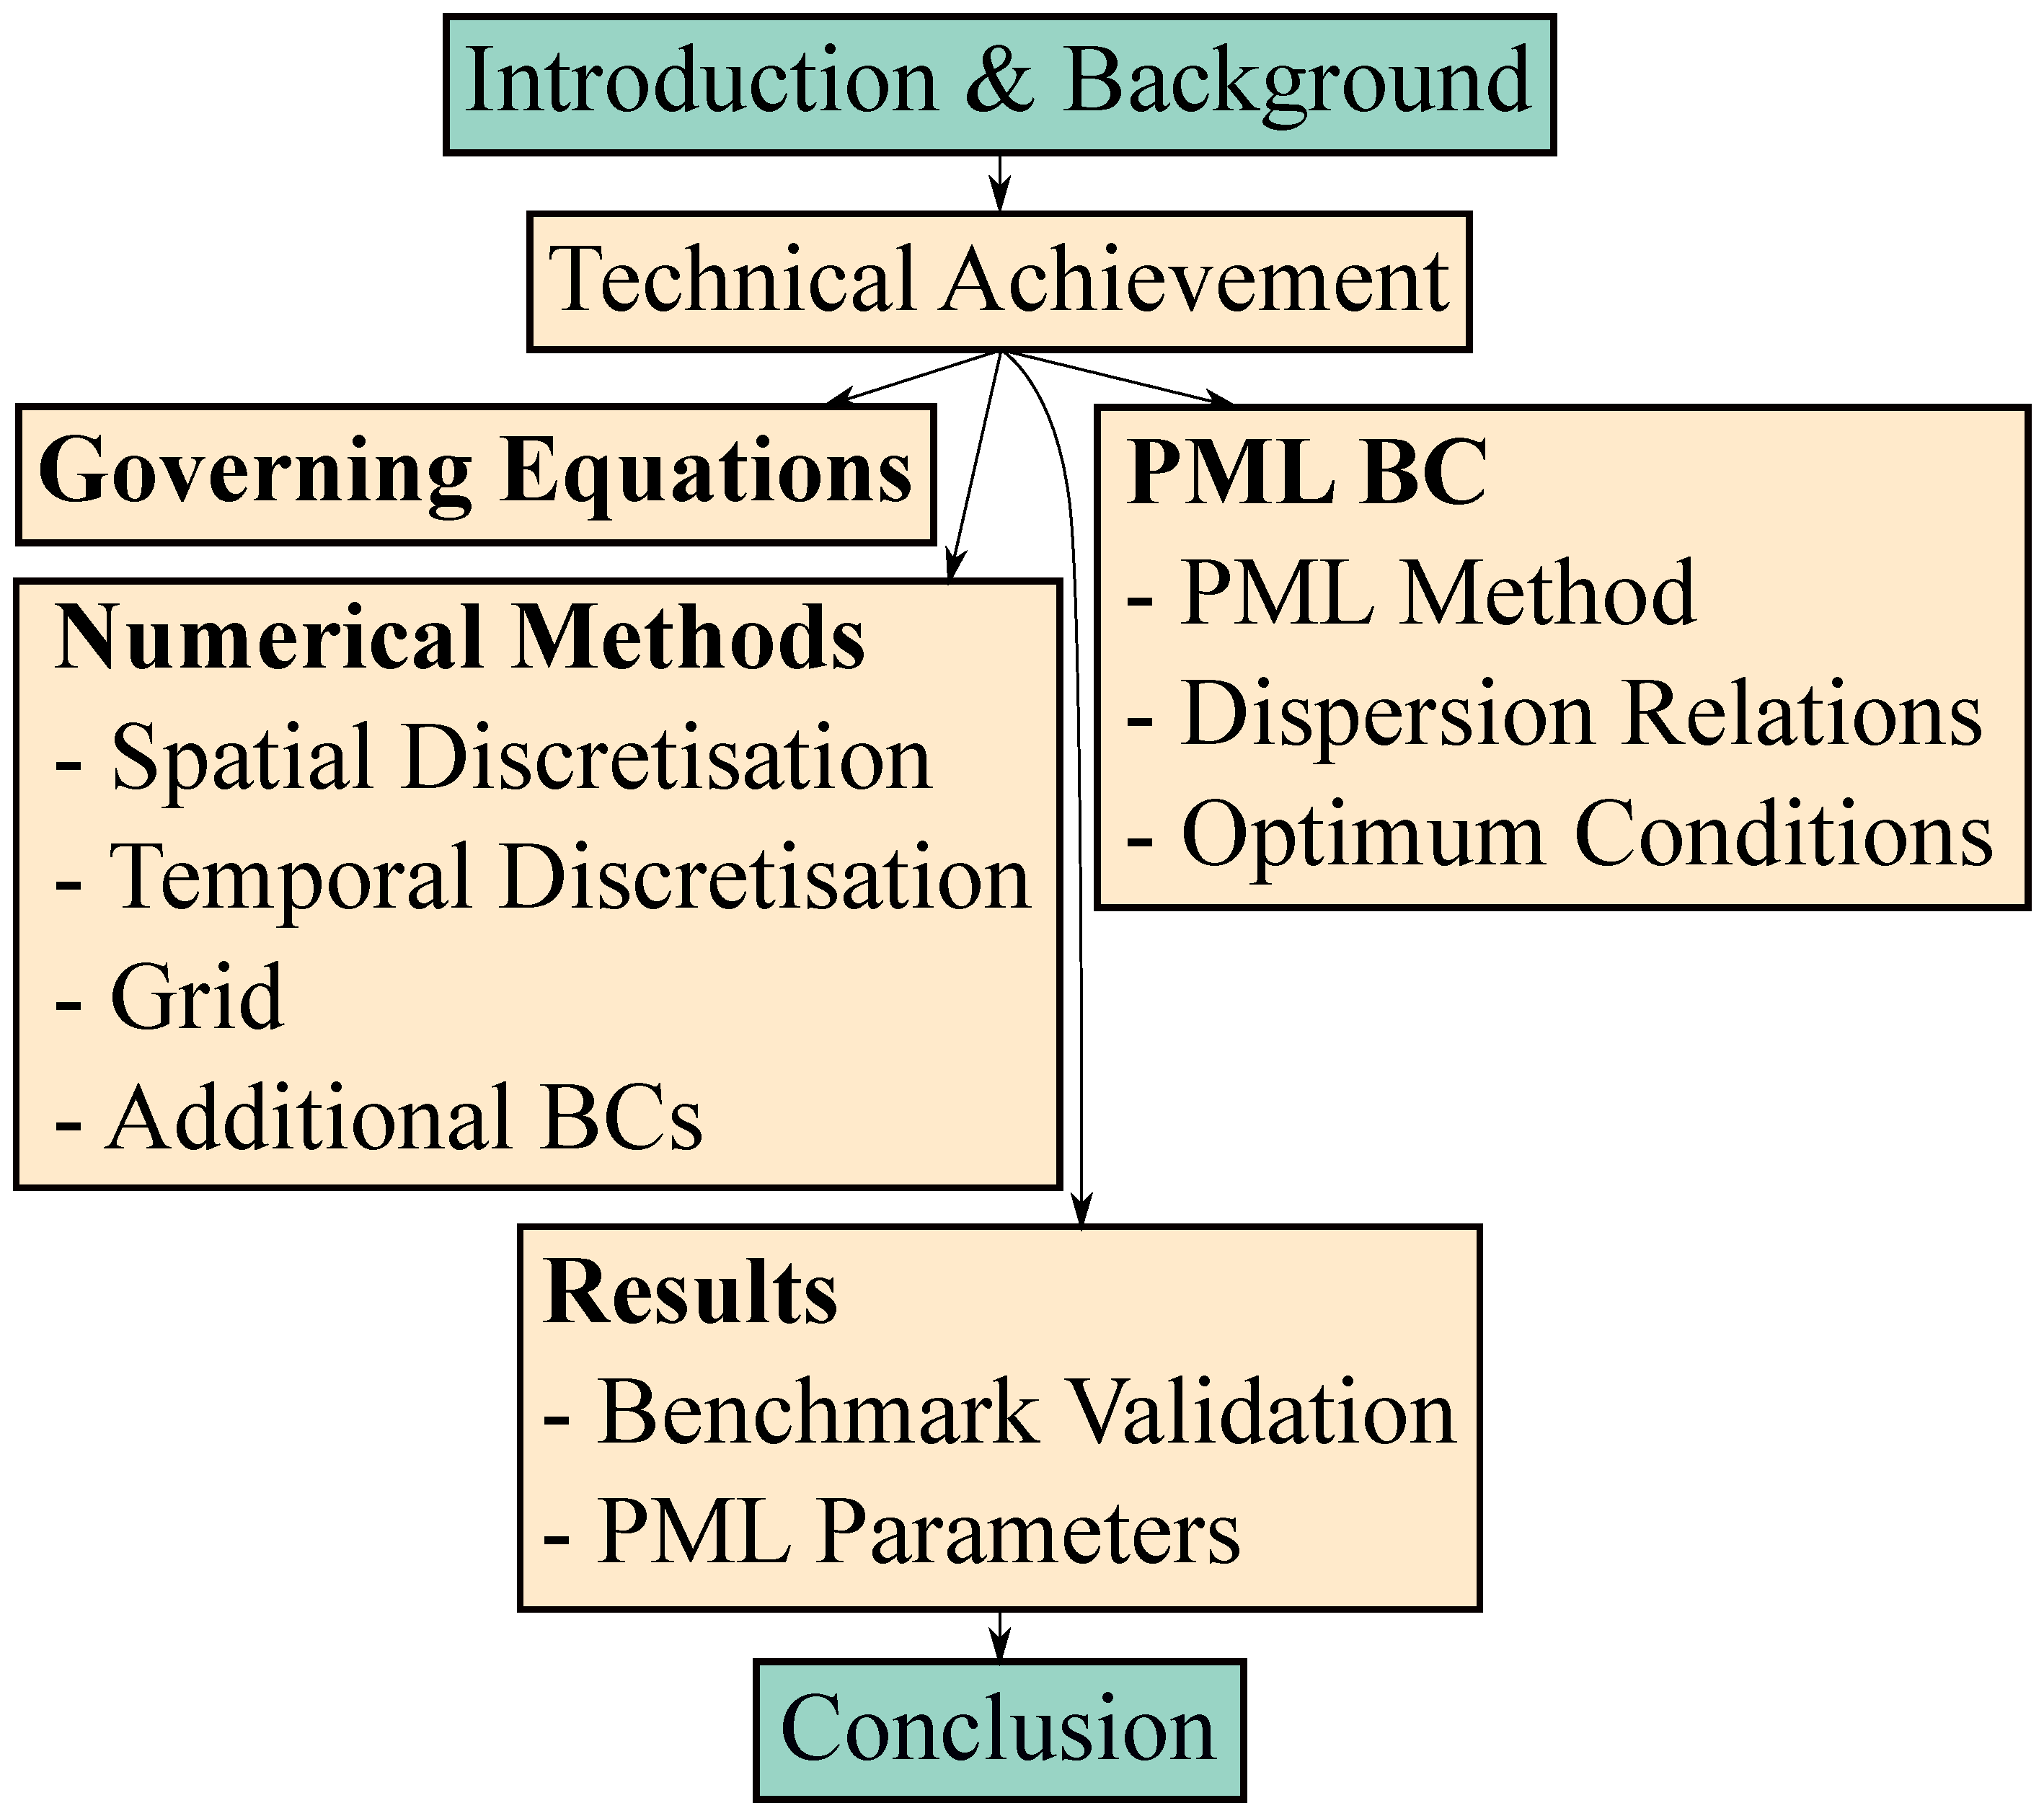
\includegraphics[width=8cm]{Figures/IntroBackground/ReportStructure.eps}}
\caption{Report Structure.}
\label{fig:ReportStructure}
\end{figure}

For methodology, first the governing Euler equations are massaged into a usable form, and then augmented with the perfectly matched layer (PML) boundary condition. The dispersion relations of two PML formulations are assessed for stability, and analytically derived optimum conditions from a source are addressed. The numerical methods for computational implementation are then compared and described, with spatial \& temporal discretisation, grid setup, and additional boundary conditions. The written solver is then validated against a set of NASA benchmark initial conditions, and then the effects of the BC parameters are investigated. The results are summarised and conclusions are drawn to deliver recommendations and further work.

4 field variables are referred to in this report: density $\rho$, velocity in the $x-$direction $u$, velocity in the $y-$direction $v$, and pressure $p$. The freestream Mach number is also defined as $M$. All other symbols are either defined as they appear, or take on their standard definition within engineering and aeroacoustics.

All figures created in this report have been the sole work of the student.